\section{环境贴图照明}\label{sec:ibl}
看图中第一排红球。两幅图都有房间里的直接光和漫反射环境光。右图又加上了环境的镜面反射，左上角原本只有小亮点的球，开始映出周围亮暗相间的形状。沿右图同一排往右看，表面越来越粗糙，倒影逐渐散开。这是 LearnOpenGL 在同一个房间里展示的两步绘制。

\begin{figure}[H]\centering
\begin{minipage}[b]{.47\linewidth}\centering
\href{https://learnopengl.com/img/pbr/ibl_irradiance_result.png}{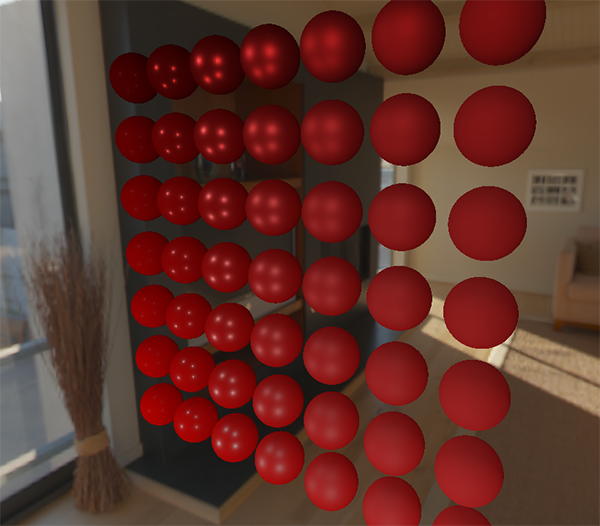
\includegraphics[height=4.85cm]{figures/ibl-diffuse-spheres.png}}\\[-1pt]
{\small 环境光只计入漫反射}
\end{minipage}\hfill
\begin{minipage}[b]{.47\linewidth}\centering
\href{https://learnopengl.com/img/pbr/ibl_specular_result.png}{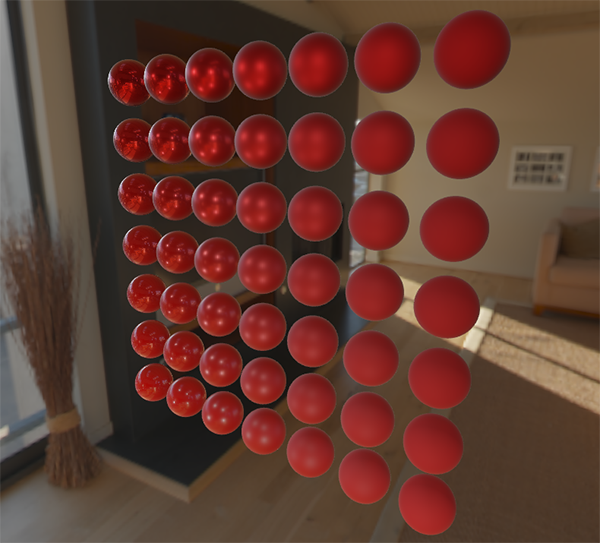
\includegraphics[height=4.85cm]{figures/ibl-specular-spheres.png}}\\[-1pt]
{\small 再加上镜面环境反射}
\end{minipage}
\caption{同一组材质球，向右粗糙度增加，向上金属度增加。两张图来自教程的不同阶段，构图略有差别，适合沿行观察。原图 © \href{https://twitter.com/JoeyDeVriez}{Joey de Vries}，LearnOpenGL 的 \href{https://learnopengl.com/PBR/IBL/Diffuse-irradiance}{Diffuse irradiance} 与 \href{https://learnopengl.com/PBR/IBL/Specular-IBL}{Specular IBL}，\href{https://creativecommons.org/licenses/by/4.0/}{CC BY 4.0}。}
\end{figure}

把相机放在这些球的位置，朝四周各拍一张照片，再朝天花板和地板各拍一张。六张图围成一个立方体，就有了一张可以按方向查颜色的环境贴图。朝窗外的方向查，读出的是窗外的光；换一个方向，同一张图便能给球的另一侧提供墙面的颜色。把这些颜色当作照明来算，就是环境贴图照明（IBL）。

在 Redflag 的 OpenGL 编辑器中，打开「渲染效果 → 环境贴图 → 载入 HDR 全景」，再勾选「环境照明 (IBL)」。全景图保留线性亮度，例如窗户可以比白墙亮许多倍。载入时，\code{IBLPrecompute} 把经纬展开的全景转成六个面，接着生成漫反射图、分粗糙度的反射图和一张材质查找表。选择同一菜单里的「保存烘焙结果」，再保存场景，下次打开就能从 \path{.rfibl} 读取这些结果。另一场景也可直接选择「使用烘焙文件」。下文讨论 OpenGL 材质着色器使用的环境光。

\subsection{表面从哪一侧受光}
先看一个没有金属成分的哑光球。球顶朝上，能收到天花板方向的光。球的侧面朝向窗户，同一扇窗对它的贡献便不同了。下图把球上一个点放大，红色法线 $N$ 标出这个点朝向哪里。

\begin{figure}[H]\centering
\href{https://learnopengl.com/img/pbr/ibl_hemisphere_sample_normal.png}{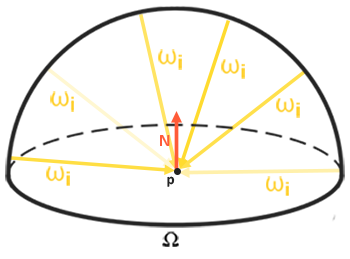
\includegraphics[height=2.65cm]{figures/effects-irradiance.png}}
\caption{只汇总表面上方半球内的来光。黄色箭头分别代表可以从环境贴图查询的来光方向。© Joey de Vries，\href{https://learnopengl.com/PBR/IBL/Diffuse-irradiance}{LearnOpenGL}，\href{https://creativecommons.org/licenses/by/4.0/}{CC BY 4.0}。}
\end{figure}

\clearpage
\subsection{光照方向与受光面积}\label{sec:ibl-card}
把一张边长 $2$ cm 的正方形卡片放在均匀的平行光下。先让卡片正对光源。从光源方向看，卡片的轮廓是一个 $2\times 2$ cm 的正方形。再绕卡片的一条边转过 $60^\circ$。卡片的大小和光源的强度都没变，但从光源看过去，轮廓变窄了。这两个轮廓画在图~\ref{fig:ibl-card} 左侧。光线平行且分布均匀，轮廓内的面积决定了卡片能截获多少光。

\begin{figure}[H]\centering
% 正方形绕一边旋转。左图沿光线看，右图沿旋转轴看。
\begin{tikzpicture}[x=1cm,y=1cm,font=\small,>=Stealth]
  \draw[rounded corners,draw=line,fill=pale!35] (0,0) rectangle (15.7,5.0);
  \draw[line] (7.45,.25)--(7.45,4.75);
  \node[anchor=west,font=\bfseries] at (.32,4.62) {沿着平行光看卡片};
  \node[anchor=west,font=\bfseries] at (7.75,4.62) {从侧面看倾斜的卡片};
  \foreach \cx/\width/\labeltext in {2.05/2/正对光源,5.48/1/转过 $60^\circ$} {
    \draw[line,dashed] (\cx-1,1.42) rectangle (\cx+1,3.42);
    \draw[fill=blue!17,draw=blue,thick] (\cx-\width/2,1.42) rectangle (\cx+\width/2,3.42);
    \draw[<->,blue] (\cx-\width/2,1.14)-- node[below] {$\width$ cm} (\cx+\width/2,1.14);
    \node at (\cx,3.82) {\labeltext};
  }
  \draw[<->,muted] (.76,1.42)--node[left] {$2$} (.76,3.42);
  \node at (2.05,.47) {$4\,\mathrm{cm}^2$};
  \node at (5.48,.47) {$2\,\mathrm{cm}^2$};
  \begin{scope}[shift={(10.7,1.02)}]
    \coordinate (a) at (0,0);
    \coordinate (b) at (1.50,2.598);
    \coordinate (c) at (1.50,0);
    \draw[fill=blue!7,draw=none] (a)--(b)--(c)--cycle;
    \draw[dashed,muted] (b)--(c);
    \draw[thick,blue] (a)--(b);
    \draw[thick,blue] (a)--(c);
    \draw[muted] (1.36,0)--(1.36,.14)--(1.50,.14);
    \draw[blue] (.57,0) arc[start angle=0,end angle=60,radius=.57];
    \node at (.95,.44) {$60^\circ$};
    \node[below] at (.75,-.05) {从光源看到的宽度};
    \node[anchor=west] at (1.66,1.7) {卡边长 $2$ cm};
    \draw[->,thick] (a)--(0,2.35) node[above] {指向光源};
    \draw[->,thick,blue] (a)--(-1.84,1.06) node[above left,inner sep=1pt] {$N$};
    \draw[muted] (0,.83) arc[start angle=90,end angle=150,radius=.83];
    \node at (-.72,1.24) {$\theta$};
  \end{scope}
\end{tikzpicture}

\caption{左图的两块蓝色区域按相同比例绘制。右图沿卡片的旋转轴看，斜边代表卡片的一条边，水平边是它从光源方向看到的宽度。$N$ 是垂直于卡片的方向，称为法线。}\label{fig:ibl-card}
\end{figure}

看右图的直角三角形。卡边和水平线的夹角是 $60^\circ$，水平边的长度等于斜边长乘以这个角的余弦，即 $2\cos60^\circ=1$ cm。沿旋转轴的那条边仍长 $2$ cm，因此卡片实际占 $4\,\mathrm{cm}^2$，沿光线看只占 $2\,\mathrm{cm}^2$。它截获的光功率也减半。这里比较的是同一张卡片，统计的始终是落在整张卡片上的光。

着色器用法线 $N$ 描述表面朝向，把法线与指向光源的方向之间的夹角记为 $\theta$。卡片转多少度，法线就转多少度，所以图中的两个角相等。换成任意面积 $A$ 的平面，沿光线看到的面积是 $A\cos\theta$。正对光源时 $\theta=0^\circ$，整个表面都能截光。光线与卡片平行时 $\theta=90^\circ$，从光源只能看到理想薄片的一条边。代码里的 \code{cos(theta)} 就来自这一步。

虎书《Fundamentals of Computer Graphics》第五版第 5 章图 5.2 把立方体的顶面转过 $60^\circ$，图 5.3 再标出法线和来光方向。图~\ref{fig:ibl-card} 是本项目重画的卡片，加上了能直接量的两条边。把倾斜面积换算为垂直于光线的面积，可接着看作者的\source{https://www.cs.cornell.edu/courses/cs6630/2022fa/notes/radiometry-notes.pdf\#page=6}{Cornell《Radiometry》讲义第 6 页}。同一现象还有一种画法，保持光束宽度，观察它在地面上照亮的面积。\source{https://pbr-book.org/4ed/Radiometry,_Spectra,_and_Color/Radiometry}{PBRT 第四版 §4.1，图 4.2}

\clearpage
\subsection{半球上的采样面积}\label{sec:ibl-sky}
现在把卡片水平放好，在卡片中心想象一个半径为 1 的半球。由中心指向窗户四个角的射线，会在球面上圈出一块区域。若同一扇窗离得更远，它在球面上圈出的范围就更小。在这个单位球上，区域的面积叫作窗户在该点所占的\textbf{立体角}，单位是球面度（sr）。环境贴图提供每个方向的来光，求总量还得知道每次查图代表多大一块球面。

\begin{figure}[H]\centering
% 球心在原点。左半图为正交投影，观察方向比赤道高 16 度。
\begin{tikzpicture}[x=1cm,y=1cm,font=\small,>=Stealth,
  declare function={skyx(\t,\p)=3.08*sin(\t)*sin(\p);
                    skyy(\t,\p)=3.08*(cos(\t)*cos(16)-sin(\t)*cos(\p)*sin(16));}]
  \draw[rounded corners,draw=line,fill=pale!35] (0,0) rectangle (15.7,5.55);
  \draw[line] (7.9,.22)--(7.9,5.3);
  \node[anchor=west,font=\bfseries] at (.32,5.17) {从半球上取两格};
  \node[anchor=west,font=\bfseries] at (8.16,5.17) {沿球轴切开，看其中一条纬线};
  \begin{scope}[shift={(4.1,1.38)}]
    \draw[line,dashed] (-3.08,0) arc[start angle=180,end angle=0,x radius=3.08,y radius=.85];
    \foreach \t in {10,20,35,45,55,65,75,90} {
      \draw[line] plot[domain=-90:90,samples=41,variable=\p] ({skyx(\t,\p)},{skyy(\t,\p)});
    }
    \foreach \p in {-90,-60,-30,-15,15,30,60,90} {
      \draw[line] plot[domain=0:90,samples=31,variable=\t] ({skyx(\t,\p)},{skyy(\t,\p)});
    }
    \foreach \ta/\tb/\col in {10/20/blue,55/65/orange!80!black} {
      \path[fill=\col!23,draw=\col,thick]
          plot[domain=-15:15,samples=13,variable=\p] ({skyx(\ta,\p)},{skyy(\ta,\p)})
       -- plot[domain=\ta:\tb,samples=8,variable=\t] ({skyx(\t,15)},{skyy(\t,15)})
       -- plot[domain=15:-15,samples=13,variable=\p] ({skyx(\tb,\p)},{skyy(\tb,\p)})
       -- cycle;
    }
    \draw[blue] ({skyx(15,-15)},{skyy(15,-15)}) -- (-1.13,2.82) -- (-1.54,2.82);
    \node[anchor=east,text=blue] at (-1.50,2.82) {近球顶};
    \draw[orange!80!black] ({skyx(60,15)},{skyy(60,15)}) -- (1.58,.74) -- (1.84,.74);
    \node[anchor=west,text=orange!80!black] at (1.79,.74) {近赤道};
  \end{scope}
  \begin{scope}[shift={(9.62,.85)}]
    \coordinate (p) at (2.60,1.5);
    \draw[line] (0,3) arc[start angle=90,end angle=0,radius=3];
    \draw[->,muted] (0,0)--(0,3.38) node[above] {球轴};
    \draw[muted] (0,0)--(3.2,0);
    \draw[very thick,blue] (0,0)--(p);
    \draw[very thick,orange!80!black] (0,1.5)--(p);
    \draw[muted] (0,1.35)--(.15,1.35)--(.15,1.5);
    \draw[muted] (0,.69) arc[start angle=90,end angle=30,radius=.69];
    \node at (.52,.89) {$\theta$};
    \node[text=blue,fill=pale!40,inner sep=1pt] at (1.47,.70) {$1$};
    \node[text=orange!80!black,above] at (1.3,1.53) {纬线半径 $r$};
    \fill[blue] (0,0) circle (1.6pt) node[below] {球心};
    \fill[orange!80!black] (p) circle (1.8pt) node[right] {球面上一点};
  \end{scope}
\end{tikzpicture}

\caption{本项目按单位球坐标绘制。两格的上下边相差 $10^\circ$，左右边相差 $30^\circ$。蓝格位于离球顶 $10^\circ$ 到 $20^\circ$ 的位置，橙格位于 $55^\circ$ 到 $65^\circ$。右图从球心向球面上的一点连线，得到斜边长为 1 的直角三角形。}\label{fig:ibl-sky}
\end{figure}

左图各条经线在球顶相遇，所以同样跨两条经线，靠近球顶的一格很窄。要算出它的宽度，先看右图。球心到球面这一段长 1，与球轴的夹角为 $\theta$。对着这个角的水平边，正好是该纬线绕球轴转一圈的半径。因此 $\sin\theta=r/1$，也就是 $r=\sin\theta$。

沿圆周走过的弧长等于半径乘转角，转角用弧度。如在半径为 1 的圆上走四分之一圈，弧长和转角都是 $\pi/2$。现在沿纬线转过很小的方位角 $\Delta\phi$，走过的宽度是 $r\,\Delta\phi$。再沿经线往下转过 $\Delta\theta$，经线所在的圆半径为 1，这一格的高度就是 $\Delta\theta$。小格的上下边略有不同，格子划得越细，用中间的宽乘高就越准确：
\[
 \Delta\omega\ \approx\
 \underbrace{(\sin\theta\,\Delta\phi)}_{\text{沿纬线的宽度}}
 \underbrace{\Delta\theta}_{\text{沿经线的高度}} .
\]
例如图中的蓝格和橙格都横跨 $30^\circ$，换成弧度是 $\pi/6$。取两格正中的纬线，蓝格的宽度是 $\sin15^\circ\times\pi/6\approx0.136$，橙格则是 $\sin60^\circ\times\pi/6\approx0.453$。两格高度相同，橙格代表的方向范围约是蓝格的 $3.35$ 倍。把小格取得无限细时，上式写作 $\mathrm d\omega=\sin\theta\,\mathrm d\theta\,\mathrm d\phi$。\source{https://pbr-book.org/4ed/Geometry_and_Transformations/Spherical_Geometry}{PBRT 第四版 §3.8.1，图 3.13}

\clearpage
\subsection{从一格来光到漫反射贴图}\label{sec:ibl-sum}
设环境贴图在一小格内的来光几乎恒定，记为 $L$，称为辐亮度。可以这样读它的单位 $\mathrm{W/(m^2\,sr)}$：沿来光方向看，每平方米的迎光面积，从每球面度的方向范围内接收多少瓦的光功率。对面积为 $A$ 的卡片，这一格带来的功率近似为 $L(A\cos\theta)\Delta\omega$。再除以卡片自身的面积 $A$，就得到单位表面积收到的功率，称为辐照度，单位为 $\mathrm{W/m^2}$。

假设环境中只有两块亮区，其余全黑。两块各占 $0.1$ sr，辐亮度均为 $2\,\mathrm{W/(m^2\,sr)}$，且亮区足够小，可用中心方向代表整块。正上方那块贡献 $2\times1\times0.1=0.2\,\mathrm{W/m^2}$。另一块中心方向与法线成 $60^\circ$，贡献 $2\times0.5\times0.1=0.1\,\mathrm{W/m^2}$。表面合计收到 $0.3\,\mathrm{W/m^2}$。照这样把所有小格加起来，便得到半球的辐照度 $E$：
\[
 E \approx \sum_i L_i\cos\theta_i\,\Delta\omega_i,\qquad
 E=\int_0^{2\pi}\!\int_0^{\pi/2}
    L(\theta,\phi)\cos\theta\,\sin\theta\,\mathrm d\theta\,\mathrm d\phi .
\]
对理想漫反射表面，从不同方向观察同一点，出射辐亮度相同。算它一共反射了多少功率，还要对各个出射方向计入图~\ref{fig:ibl-card} 的余弦。先沿经线相加。令 $u=\sin\theta$，因为正弦的导数是余弦，便有 $\mathrm du=\cos\theta\,\mathrm d\theta$。从球顶走到赤道时，$u$ 从 0 增至 1，于是
\[
\int_0^{\pi/2}\sin\theta\cos\theta\,\mathrm d\theta
=\int_0^1 u\,\mathrm du=\tfrac12 .
\]
最后这个数也能从图形读出：直线 $y=u$ 在 0 到 1 之间围出的面积，是底和高都为 1 的三角形面积。绕半球一周有 $2\pi$ 弧度，各条经线的积分相同，总和便是 $2\pi\times\tfrac12=\pi$。若表面反射收到光的比例为 $\rho$，每个方向的出射辐亮度就应取 $\rho E/\pi$。Redflag 把 $E/\pi$ 存入漫反射贴图，绘制材质时再乘底色。\source{https://openstax.org/books/calculus-volume-1/pages/5-5-substitution}{OpenStax《Calculus》卷一 §5.5，换元积分}

GPU 给贴图的每个输出像素选一个法线方向。下面是其中一个像素的计算，循环内的 \code{w} 从表面指向环境。第一次乘法计入面的朝向，第二次计入这一格的球面面积。两个角度的步长固定，因此可以在循环结束时统一处理。
\begin{lstlisting}
for (int column = 0; column < azimuthSteps; ++column) {
    float phi = (column + 0.5) * (2.0 * PI / azimuthSteps);
    for (int row = 0; row < polarSteps; ++row) {
        float theta = (row + 0.5) * (0.5 * PI / polarSteps);
        // 此处略去把格子中心的两个角度换算成世界方向 w 的代码。
        irr += texture(u_EnvMap, w).rgb * cos(theta) * sin(theta);
    }
}

// 循环结束后乘角度步长，再除以理想漫反射的圆周率因子。
irr = PI * irr / float(polarSteps * azimuthSteps);
\end{lstlisting}
\loc{Redflag/src/Redflag/Renderer/IBLPrecompute.cpp}{s\_IrradianceFS（循环内累加，循环后归一化）}
若共有 $n$ 个等角度采样点，每点代表的\emph{角度步长乘积}约为 $(2\pi)(\pi/2)/n=\pi^2/n$。把它乘入总和，再除以漫反射的 $\pi$，就有了代码最后的 $\pi/n$。可用一张纯色环境图检查：若每个方向的输入都是 $L$，就有 $E=\pi L$，输出贴图应在离散近似的误差内还原 $L$。\source{https://learnopengl.com/PBR/IBL/Diffuse-irradiance}{LearnOpenGL · Diffuse irradiance}

用线性颜色 $(2,1,0.5)$ 做这项检查时，旧版读回约 $(1.9941,0.9971,0.4985)$。它从每格的起始边缘取样，最后一格还跨过半球的边缘。现在把四分之一圈等分成 63 行，一整圈等分成 252 列，每一格都在中心取样，代码中的 $+0.5$ 表示从格边向内走半格。两次都查 $63\times252=15{,}876$ 个方向，新版在六个面的全部 $6\times32^2$ 个半精度像素上读回 $(2,1,0.5)$。误差小到这张贴图的精度已分辨不出。

\clearpage
\subsection{粗糙度与环境倒影}
再看房间的窗框。把最左边展开的立方体和右边逐渐缩小的几张图放在一起，窗框的轮廓从清晰到模糊。每一层都对多个方向的光做了加权平均，表面越粗糙，参与平均的方向范围越宽。
\begin{figure}[H]\centering
\href{https://learnopengl.com/img/pbr/ibl_prefilter_map.png}{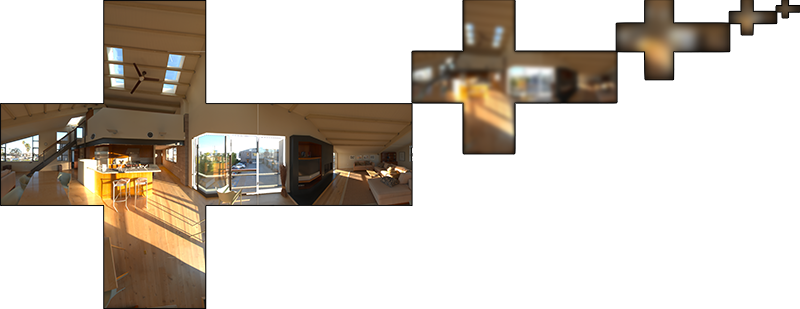
\includegraphics[width=.76\linewidth]{figures/ibl-prefilter-map.png}}
\caption{从左向右看十字形环境贴图，留意房间中央的窗。黑色是六个面展开后留下的空位。© \href{https://twitter.com/JoeyDeVriez}{Joey de Vries}，\href{https://learnopengl.com/PBR/IBL/Specular-IBL}{LearnOpenGL · Specular IBL}，\href{https://creativecommons.org/licenses/by/4.0/}{CC BY 4.0}。}
\end{figure}

原本，每个着色点都要把来光颜色与材质对该方向的反射比例相乘，再对各方向求和。Epic 的 Brian Karis 将这一步近似拆成两份预计算。第一份就是上图，只保留环境、倒影方向和粗糙度。生成它时假设视线、法线和反射方向重合，因此掠过表面的狭长倒影会有误差。第二份只与材质有关，存成一张二维表，横轴是法线与视线夹角的余弦，纵轴是粗糙度。

这张表只要两个数。把 Fresnel 近似写成 $F=F_0(1-c)+c$，其中 $c=(1-V\cdot H)^5$，$H$ 是能把光反射进视线的微表面法线。每个样本的可见度和采样权重记为 $w_i$。把材质正面反射率 $F_0$ 提到求和号外，就得到
\[
 \frac1n\sum_i w_i F_i =
 F_0\underbrace{\frac1n\sum_i w_i(1-c_i)}_{a}
 +\underbrace{\frac1n\sum_i w_i c_i}_{b}.
\]
Redflag 的 \code{IntegrateBRDF} 将 $a,b$ 写入红、绿通道。着色时项目用包含粗糙度修正的 \code{kS} 作为反射颜色。先算相机在表面的镜面方向 \code{R}，再按粗糙度取一层房间的倒影，用查表结果调整它的强度。
\begin{lstlisting}
// 先求镜面方向，再按粗糙度选取相应的反射图层。
vec3 R = reflect(-V, N);
vec3 prefilteredColor = textureLod(u_PrefilterMap, R, roughness * MAX_REFLECTION_LOD).rgb;
vec2 brdf = texture(u_BRDFLUT, vec2(max(dot(N, V), 0.0), roughness)).rg;
vec3 reflection = kS * brdf.x + brdf.y;
\end{lstlisting}
\loc{RedflagForge/assets/shaders/Renderer3D_Mesh.glsl}{main（节选）}
系数 4 来自五层反射图，层号从 0 到 4。粗糙度为 0.5 时取第 2 层。最后按 \code{ambient = (kD * diffuseIBL + specularIBL) * ao} 合成；这里把遮蔽同时乘到漫反射和镜面项，是项目采用的近似。\source{https://blog.selfshadow.com/publications/s2013-shading-course/karis/s2013_pbs_epic_notes_v2.pdf}{Brian Karis，SIGGRAPH 2013 课程笔记，第 5--7 页}


\clearpage
\subsection{粗糙金属的环境反射}
把金属球放进四周同样明亮的房间。假设光源的线性亮度是 1，球面也不吸收任何光，那么无论球面如何打磨，最终看到的亮度都应是 1。这种测试环境叫白炉（white furnace）。在下图左半，第一排最右端的球却明显变暗。前面的计算只追踪光在一块微小表面上反射之后直接离开。表面越粗糙，反射光越容易先撞上旁边的表面。这部分光有机会经过几次反射后离开。

\begin{figure}[H]\centering
{\small\makebox[.43\linewidth]{只计算一次反射}\makebox[.43\linewidth]{补回粗糙金属的反射}}\\[3pt]
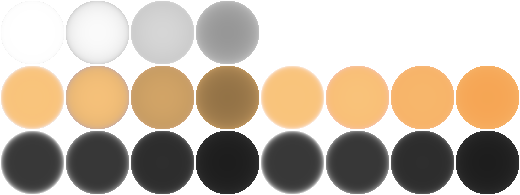
\includegraphics[width=.86\linewidth]{../../../output/validation/metal-furnace/vulkan.png}
\caption{Redflag Vulkan 计算着色器输出。左侧四列为旧版，右侧四列为修正后。每组从左至右的粗糙度为 0.1、0.4、0.7、1。上排是理想白金属，中排是有色金属，下排是底色为黑的塑料。上排修正后融入白色背景，表示它把收到的光都反射了回来。}
\end{figure}

仍用上一页的查询表。对白金属，$F_0=1$，查表返回的 $E=a+b$ 就是经过一次反射后已经离开的比例。在粗糙度为 1 的球面中央，我们读到了 $E=0.30814$。白金属应该完整反射，所以还要补回 $1-E$。有色金属每次反射都会吸收一部分光，并且三个颜色通道的吸收不同。Turquin 的近似让每个通道按自身的 $F_0$ 补偿。写 $m$ 为材质的金属度，$S=k_Sa+b$ 为原反射颜色，Redflag 作用于环境倒影的计算为
\[
  S' = S + mF_0\bigl(S/E-S\bigr).
\]
取 $m=F_0=1$ 得 $S'=1$；取 $m=0$ 得 $S'=S$。有色金属这一排取 $F_0=(0.95,0.55,0.20)$，最粗糙球的中心由 $(0.293,0.169,0.062)$ 变为 $(0.917,0.379,0.089)$，看起来仍保留金属自身的颜色。这个近似沿用原反射图层，因此不会产生环境图本身没有的倒影。

\begin{lstlisting}
// 两个通道相加，得到同样粗糙的白金属经过一次反射后返回的比例。
float singleBounce = brdf.x + brdf.y;
if (singleBounce > 0.0)
    reflection += metallic * F0 * (reflection / singleBounce - reflection);
vec3 specularIBL = prefilteredColor * reflection;
\end{lstlisting}
\loc{RedflagForge/assets/shaders/Renderer3D_Mesh.glsl}{main（片元阶段节选）}
Vulkan 的 \code{specularEnvironment} 使用相同的两个通道。两条路径都对准同一张表和同一片球面，白金属最大误差为 $1.2\times 10^{-7}$。将环境光调为黑色，球面上所有材质也都返回 0。\source{https://google.github.io/filament/main/filament.html}{Filament，Energy compensation 与 Pre-integration for multiscattering}

\clearpage
\subsection{全景图的接缝}
把纸上的世界地图卷成圆筒，最左列和最右列便成了邻居。全景图也如此。为了看清纹理过滤有没有跨过这条缝，测试只用四列像素，前两列亮、后两列暗。选取红通道，亮处设为 1，暗处设为 0。两列正中间应各取一半，得到 0.5。

\begin{figure}[H]\centering
\begin{tabular}{@{}r@{\quad}c@{}}
旧版 & \fbox{
\includegraphics[width=.70\linewidth,height=8mm]{figures/ibl-seam-before.png}}\\
修正后 & \fbox{
\includegraphics[width=.70\linewidth,height=8mm]{figures/ibl-seam-after.png}}
\end{tabular}
\caption{实机 OpenGL 读回。两条带都取自环境立方体负 $X$ 面正中的同一行，横向覆盖该面的 2048 个像素。线性红通道从 0 到 1 直接映射为黑到白，纵向重复同一行以便观察。上下两条的正中央是同一条经线。}
\end{figure}

旧版在纹理的左右两端分别钳住边缘像素，显卡读到接缝两侧为 1 和 0。把经度方向改为循环取样后，两侧实测都为 0.5。上下边缘仍分别位于北极和南极，因此纬度方向继续钳住。项目中这两行只作用于读入的二维全景图。
\begin{lstlisting}
// 左右两列在经度接缝处相邻，上下两端各自位于一个极点。
glTexParameteri(GL_TEXTURE_2D, GL_TEXTURE_WRAP_S, GL_REPEAT);
glTexParameteri(GL_TEXTURE_2D, GL_TEXTURE_WRAP_T, GL_CLAMP_TO_EDGE);
\end{lstlisting}
\loc{Redflag/src/Redflag/Renderer/IBLPrecompute.cpp}{IBLPrecompute::Init}
同一张测试图还在绿通道埋入一个更亮的输入：128 与 0 的中点应为 64。旧版上传前把大于 50 的亮度都压到 50，接缝两侧实际读到 50 和 0。现在输入保留到半精度浮点纹理的最大有限值 65504，修正后读到 64 和 64。65504 来自纹理格式；原先的 50 是为抑制孤立亮点设的经验值，会一并削弱光源本身。最后显示时再做色调映射。

在仓库根目录运行 \path{tests/run_ibl_tests.cmd} 可检查两个接缝值。另一项用例将六个面的输入都设成 $(2,1,0.5)$，核对漫反射图和五层镜面图是否都能保住这块纯色。前者检查方向相邻的两列怎样混合，后者检查上一节积分的归一化。
